\documentclass[11pt]{article}
\usepackage[utf8]{inputenc}
\usepackage{graphicx}
\usepackage[left=1.8cm, right=1.8cm, top=2cm, bottom=1.8cm]{geometry}
\usepackage{tabularx}
\usepackage{pbox}
\usepackage{physics}
\usepackage{caption}
\usepackage{booktabs}
\usepackage{fancyhdr}
\usepackage{enumitem}
\usepackage{multirow}
\usepackage{algorithm}
\usepackage{algpseudocode}
\usepackage{ctable}
\usepackage{appendix}
\usepackage{amssymb}
\usepackage[medium]{titlesec}
\usepackage{wrapfig}
\titleformat*{\section}{\Large\bfseries}
\titleformat*{\subsection}{\large\bfseries}
\usepackage[font=small,skip=0pt]{caption}
\setlength{\textfloatsep}{2pt}
\pagestyle{fancy}


\title{Analyse Numérique : Devoir 4}
\author{Valentin Lemaire}
\date{9 décembre 2019}

\begin{document}
\rhead{Valentin Lemaire - 16341700}
\lhead{Devoir 4 : GMRES préconditionné}
\vspace{-10pt}
\section{Analyse de convergence}\label{convsec}
\vspace{-10pt}
Grâce à l'algorithme \ref{GMRESalgo} décrit en Annexe \ref{GMRESannex}, il est possible de résoudre, de manière itérative, des systèmes linéaires et notamment ceux du modèle \texttt{ndt.py}. L'intérêt de cette méthode, comparée aux méthodes directes est le choix d'un critère d'arrêt lié (indirectement) à la précision de la solution comme discuté en section \ref{qualitysec}. En effet la fonction prend en argument un paramètre \texttt{rtol} qui va servir à comparer les résidus à chaque itération et a arrêter l'algorithme si celui-ci atteint une valeur inférieure à \texttt{rtol}. \\
\vspace{-8pt}

Les procédés iteratifs ont de nombreux avantages mais pour en vérifier la qualité il faut tout d'abord s'assurer de sa convergence. Les graphes en figures \ref{gmresconvsmall} et \ref{gmresconvbig} montrent le taux de convergence de cet algorithme pour les 4 régimes avec et sans préconditionnement pour un grand maillage petit maillage (393 noeuds) et un grand maillage (2008 noeuds) respectivement. Ces graphes ont été générés avec une valeur de \texttt{rtol = 1e-11} et une limite du nombre d'itérations maximales à 300\footnote{En pratique, \texttt{rtol} n'est pas si bas (et varie plutôt entre $10^{-6}$ et $10^{-10}$) et les itérations sont arrêtées avant d'arriver à une solution qui ne s'améliore plus, auquel cas la technique de restart est lancée.}.\\[10pt]
\begin{minipage}{0.35\textwidth}
   
   Comme le montrent ces graphes, l'algorithme converge bien. En effet, à chaque itération, la norme du résidu relatif est inférieur au précédent. Et ce, quel que soit le régime et la taille de la matrice. Ceci correspond au résultat attendu puisqu'à chaque itération de GMRES, la norme du résidu est minimisée sur un espace de plus en plus grand (l'espace de Krylov gagne une dimension à chaque itération). Dès lors, la minimisation d'une même quantité sur un espace plus grand ne peut être inférieure à la minimisation sur un sous-espace. \\
\end{minipage}
\begin{minipage}{0.65 \linewidth}
    \centering
    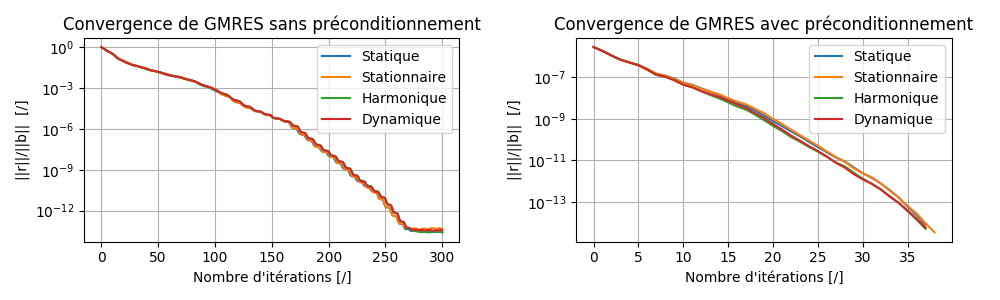
\includegraphics[width=\linewidth]{gmres_conv_small.png}
    \captionof{figure}{Convergence de GMRES pour un petit maillage}
    \label{gmresconvsmall}
        
    \centering
    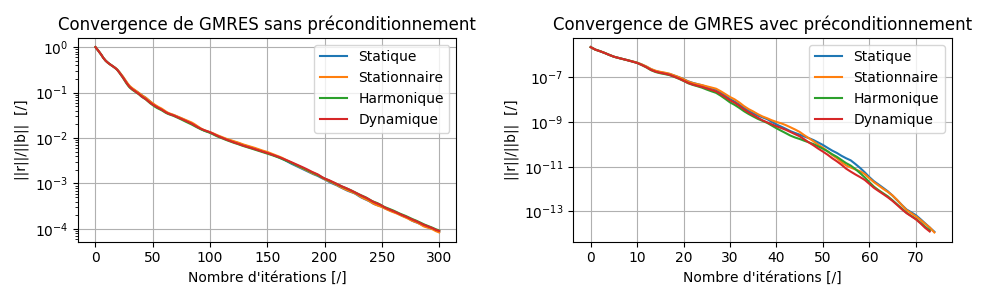
\includegraphics[width=\linewidth]{gmres_conv_big.png}
    \captionof{figure}{Convergence de GMRES pour un grand maillage}
    \label{gmresconvbig}
\end{minipage}

\begin{wrapfigure}[18]{r}{0.25\linewidth}
\vspace{-8pt}
    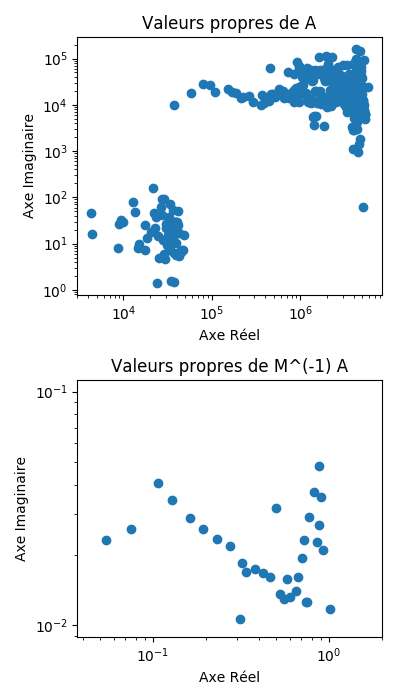
\includegraphics[width=\linewidth]{valpropr.png}
    \caption{Valeurs propres}
    \label{valsing}
\end{wrapfigure}

Pour les grand maillages la norme du résidu commence par baisser mais après un certain nombre d'itérations, ne s'améliore plus (ou alors le nombre d'itérations dépasse 300 et l'algorithme s'arrête). Ceci est dû aux erreurs numériques et à un certain moment les propriétés de l'espace de Krylov se détériorent et la solution ne s'améliore plus. C'est pourquoi en pratique la technique de restart est implémentée. \\
\vspace{-8pt}



Ces graphes présentent de grandes différences entre l'algorithme qui utilise le préconditionnement et celui qui ne le fait pas, ceci est discuté en section \ref{precsec}.
\vspace{-10pt}
\section{Effet du préconditionnement}\label{precsec}
\vspace{-10pt}
Les graphes en figures \ref{gmresconvsmall} et \ref{gmresconvbig} montrent que l'algorithme converge beaucoup plus vite lorsque la technique de préconditionnement est appliquée. En effet, pour les deux maillages, le critère de convergence est obtenu en quelques dizaines d'itérations avec préconditionnement, tandis que sans, le critère de convergence n'est toujours pas atteint après plusieurs centaines d'itérations. \\
\vspace{-8pt}

Ceci montre clairement que l'algorithme GMRES préconditionné offre un taux de convergence bien meilleur que GMRES sans préconditionnement. Ceci s'explique par le fait que lorsque le système est précondtionné, c'est $M^{-1}A x = M^{-1}b$ qui est résolu plutôt que $A x = b$. Or, comme vu au devoir 2, le conditionnement de $M^{-1}A$ est plus faible de plusieurs ordres de grandeur que le conditionnement de $A$. Et comme le taux de convergence de l'algorithme GMRES est régi par le conditionnement du problème et la répartition des valeurs propres. Au plus faible est le conditionnement et au plus les valeurs propres sont rassemblées, au plus l'algorithme convergera vite. \\
\vspace{-8pt}

La figure \ref{valsing} montre cette répartition des valeurs propres pour le régime dynamique ($f = 50Hz, vel = 1m/s$) et un maillage de 393 noeuds.  Il est clair que les valeurs propres de $M^{-1} A$ sont rassemblées et très proche les unes des autres par rapport à celles de la matrice $A$. Ceci entrainera une meilleure convergence.
\vspace{-10pt}

\section{Qualité de la solution}\label{qualitysec}
\vspace{-8pt}
Les deux sections précédentes montrent que l'algorithme converge et qu'il converge plus rapidement si la matrice est préconditionnée. Cependant, il reste à montrer que la solution vers laquelle l'algorithme converge est bien celle attendue. Une première approche est de regarder la valeur de la précision relative : $\frac{||Ax - b||_2}{||b||_2}$. Le tableau \ref{regimescomp} reprend les précisions relatives et le nombre d'itérations pour les 4 régimes quand le système est préconditionné (1) ou pas (2) lorsqu'on applique l'algorithme avec un \texttt{rtol = 1e-7} avec un maillage de 393 noeuds. \\
\vspace{-12pt}
\begin{table}[h!]
\centering
\begin{tabular}{|c|c||c|c|c|c|}
    \hline
     \multicolumn{2}{|c||}{}   & \textbf{Statique} & \textbf{Stationnaire} & \textbf{Harmonique} & \textbf{Dynamique} \\
     \multicolumn{2}{|c||}{}   & \texttt{f=0, vel=0} & \texttt{f=0, vel=1} & \texttt{f=50, vel=0} & \texttt{f=50, vel=1} \\
    \hline
    \multirow{2}{*}{(1)} & \textbf{Précision} [/] & $8.39 \cdot 10^{-5}$  & $6.37 \cdot 10^{-5}$  & $8.45 \cdot 10^{-5}$  & $5.68 \cdot 10^{-5}$ \\ \cline{2-6}
    & \textbf{Nombre d'itérations} [/] & 25 & 26  &  24 & 25\\
    \hline
    \multirow{2}{*}{(2)} & \textbf{Précision} [/] & $7.17 \cdot 10^{-11}$ & $7.40 \cdot 10^{-11}$ & $7.07 \cdot 10^{-11}$ & $8.35 \cdot 10^{-11}$\\ \cline{2-6}
    & \textbf{Nombre d'itérations} [/] & 232  & 233 & 235 & 234\\
    \hline
\end{tabular}
\caption{Précisions pour les 4 régimes}
\label{regimescomp}
\end{table}
\vspace{-10pt}

\begin{wrapfigure}[13]{r}{0.4\linewidth}
\vspace{-8pt}
    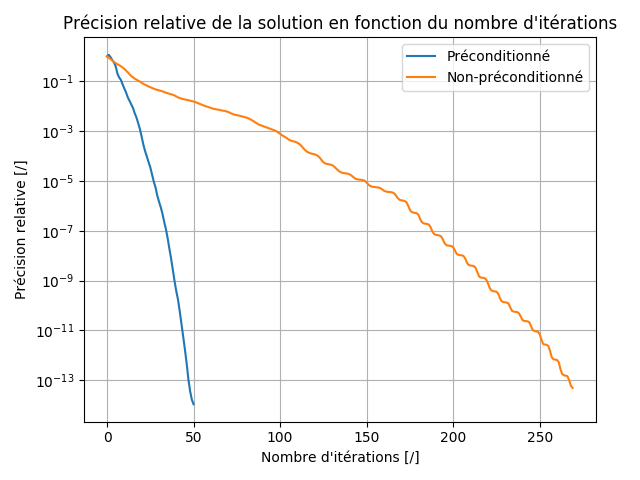
\includegraphics[width=\linewidth]{preciter.png}
    \caption{Précision relative selon les itérations}
    \label{preciter}
\end{wrapfigure}
La solution converge donc vers une solution et la précision relative est excellente dans le cas du système non-préconditionné. Dans le cas du préconditionné, elle est bonne mais pas aussi bonne. Ceci vient du fait que pour le modèle préconditionné, le résidu est calculé avec $||M^{-1}(Ax-b)||_2$. et donc le résidu est une combinaison linéaire de $Ax-b$ mais comme les valeurs singulières de $M^{-1}$ sont inférieures à l'unité\footnote{Dans le modèle \texttt{ndt}, la matrice $A$ le module des valeurs singulières de l'ordre de $10^3$ à $10^6$, et comme $M$ est la décomposition ILU(0) de $A$, $M \approx A$ et donc les valeurs singulières de $M^{-1}$ sont approximativement égales à l'inverse de valeurs singulières de $A$ et donc inférieures (en module) à 1.}, $||M^{-1}(Ax-b)||_2 < ||Ax-b||_2$. La norme du résidu du système préconditionné sera toujours inférieure à la précision du problème et donc la précision relative sera moins bonne pour un système préconditionné que pour un système non-préconditionné avec le même \texttt{rtol}.  Il convient donc de se demander si une meilleure précision peut être obtenue avec un \texttt{rtol} plus faible et un plus grand nombre d'itérations (mais qui resterait inférieur à celui du système non-préconditionné). Le graphe \ref{preciter} montre la précision relative obtenue en fonction du nombre d'itérations réalisées par GMRES (avec 393 inconnues et en régime dynamique). Celui-ci montre clairement qu'une bonne précision peut être obtenue en baissant le paramètre \texttt{rtol} et ce en un nombre considérablement plus petit d'itérations que s'il n'y a pas préconditionnement. \\
\vspace{-8pt}

La précision relative donne une bonne idée de la qualité de la solution si le problème est bien posé. Il est également intéressant de voir si la solution s'approche de la solution exacte $x^*$. En prenant la solution donnée par le solveur de numpy comme solution exacte $x^*$, il est possible d'analyser $\frac{||x-x^*||_2}{||x^*||_2}$ qui donne une idée de la proximité de la solution obtenue par rapport à la solution exacte. Cette analyse montre que pour tous les régimes et toutes les tailles de noeuds, au plus \texttt{rtol} est faible au plus on se rapproche de la solution exacte (jusqu'au moment où la solution ne converge plus, cfr. section \ref{convsec})

\newpage
\appendices
\section{Annexe : Algorithme GMRES avec préconditionnement}\label{GMRESannex}
L'algorithme GMRES avec préconditionnement peut s'écrire comme suit. Considérons la résolution du système linéaire $Ax = b$. ILU(0) est utilisé comme préconditionneur et $M$ est la décomposition ILU(0) de $A$ : $M = \hat{L}\hat{U}$. L'itéré initial est $u_0 = 0$, sauf si le restart est implémenté, auquel cas il peut être non-nul.

\begin{algorithm}
\caption{Algorithme GMRES préconditionné}\label{GMRESalgo}
\begin{algorithmic}
\State $r_0 = M^{-1}(b - A u_0)$ ;  $\beta = ||r_0||_2$; $v_1 = r_0/\beta$ \Comment{M est la décomposition ILU(0) de A : $M = \hat{L}\hat{U}$}

\For{m = 1, 2, ..., max\_iter}
    \State $w = M^{-1} A v_m$ \Comment{Multiplication par $M^{-1}$ se fait en résolvant le système $\hat{L}\hat{U}w = Av_m$}
    \For{i = 1, .., j}
        \State $h_{i, m} = v_i^* w$
        \State $w = w - h_{i, m}v_i$
    \EndFor
    \State $h_{m+1, m} = ||w||_2$
    \State $v_{m+1} = w / h_{m+1, m}$
    \State
    \State $V_m = [v_1, v_2, ..., v_m]$ ; $\bar{H}_m = [h_{i, j}]$\Comment{$\bar{H}_m$ est $[h_{i, j}]$ pour $i = 1, 2,...,m+1$ et $j = 1, 2, ..., m$}
    \State $\min\limits_{y \in \mathbb{R}^m} ||\beta e_1 - \bar{H}_my||_2$ ( $ = || r_m||_2)$ \Comment{Fait avec la décomposition QR}
    \State
    \If {$||r_m||_2 < rtol$}
        \State break
    \EndIf
\EndFor
\If{$||r_m||_2 > rtol$}
    \State $u_0 = u_0 + V_m y$
    \State restart
\EndIf
\State $u = u_0 + V_m y$
\end{algorithmic}
\end{algorithm}

\vspace{12pt}
A l'itération $n$ de cet algorithme, les vecteurs et matrices suivants sont maintenus en mémoire. Notons $N$ le nombre d'inconnues du système ($A$ est de dimension $N \cross N$). 
\begin{itemize}
    \item Tout au long de l'algorithme, $u_0$, $b$ et $r_0$ ne changent pas et sont des vecteurs de taille $N$. $A$ est une matrice de taille $N \cross N$ (sauvegardée sous format CSR), $\beta$ est un scalaire. $M$ est une matrice sous format CSR qui représente une matrice de taille $N \cross N$ et qui est représentative des matrices $\hat{L}$ et $\hat{U}$, le résultat de la décomposition ILU(0) de $A$.
    \item Ensuite, certaines variables qui dépendent de l'itération. $||r_n||_2$ est un scalaire représentant la norme du résidu de la solution par rapport au système à l'itération $n$. $w$ est un vecteur de taille $N$.
    \item Il y a également la matrice $\bar{H}_n$ qui est de dimension $(n+1) \cross n$ (et qui est donc plus grande à chaque itération).
    \item La matrice $V_n$ de dimension $N \cross n$ ($n$ vecteurs de dimension $N$). 
    \item $e_1$ est un vecteur de dimension $n+1$ est tel que $e_1 = [1, 0, 0, ..., 0]^T$ et donc $y$ est un vecteur de dimension $n$ et est la solution du problème de minimisation par les moindres carrés. 
    \item Si $n$ était la dernière itération, on va appliquer le produit $V_n y$ qui donnera un vecteur de taille $N$ (qu'on additionne à $u_0$) pour donner le vecteur solution $u$ de taille $N$ également
\end{itemize}
\end{document}